\documentclass{article}
\usepackage{graphicx}
\title{Sprawozdanie}
\author{Michal Safuryn, Bartosz Smolibowski, Wojciech Balcer}
\date{\today}
\begin{document}
\maketitle
\section{Parki}
\begin{figure}[h!]
\centering
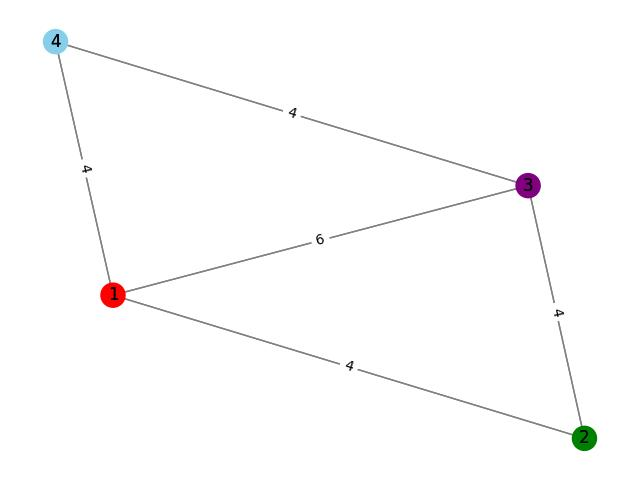
\includegraphics[width=0.75\textwidth]{1.jpg}
\caption{Park numer 1}
\end{figure}
\begin{figure}[h!]
\centering
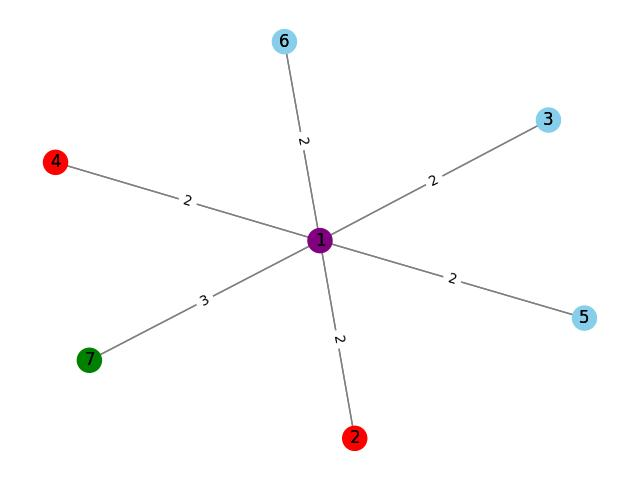
\includegraphics[width=0.75\textwidth]{2.jpg}
\caption{Park numer 2}
\end{figure}
\begin{figure}[h!]
\centering
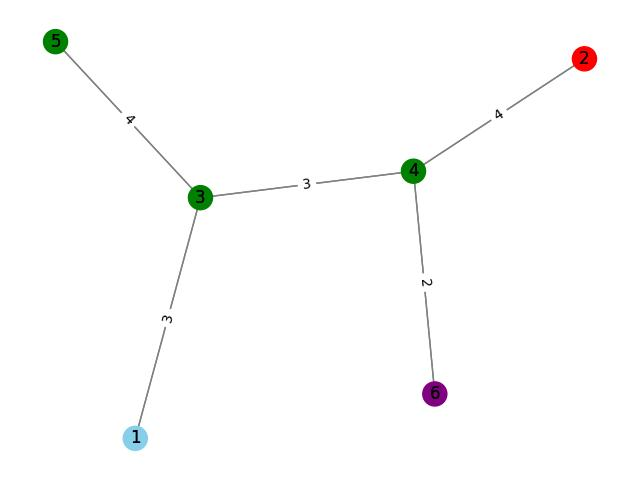
\includegraphics[width=0.75\textwidth]{3.jpg}
\caption{Park numer 3}
\end{figure}
\begin{figure}[h!]
\centering
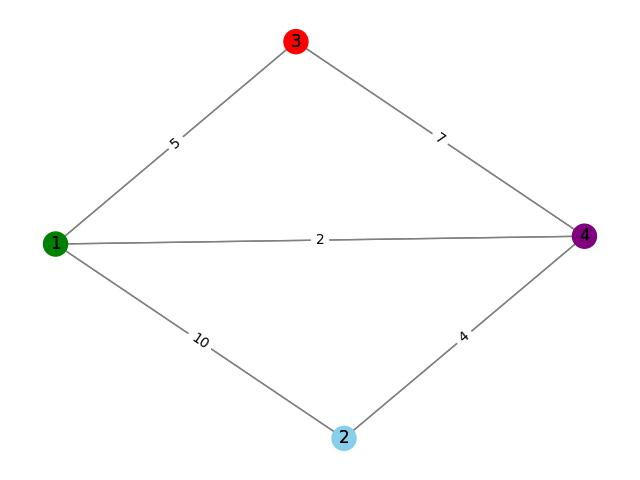
\includegraphics[width=0.75\textwidth]{4.jpg}
\caption{Park numer 4}
\end{figure}
\begin{figure}[h!]
\centering
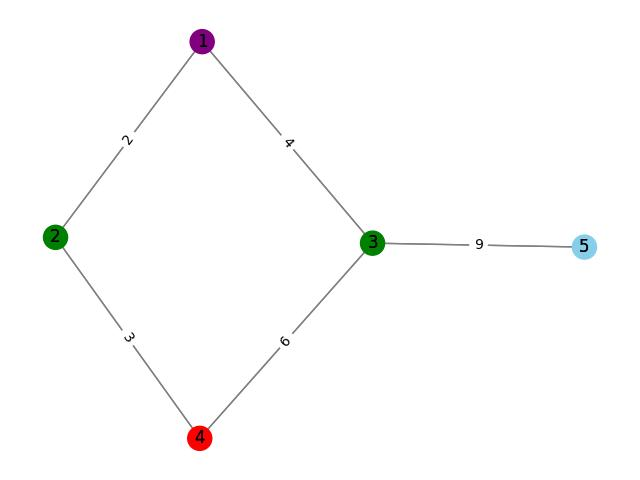
\includegraphics[width=0.75\textwidth]{5.jpg}
\caption{Park numer 5}
\end{figure}
\begin{figure}[h!]
\centering
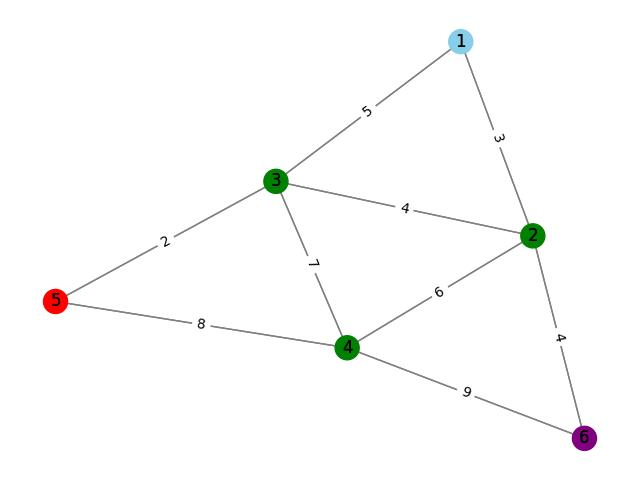
\includegraphics[width=0.75\textwidth]{6.jpg}
\caption{Park numer 6}
\end{figure}
\begin{figure}[h!]
\centering
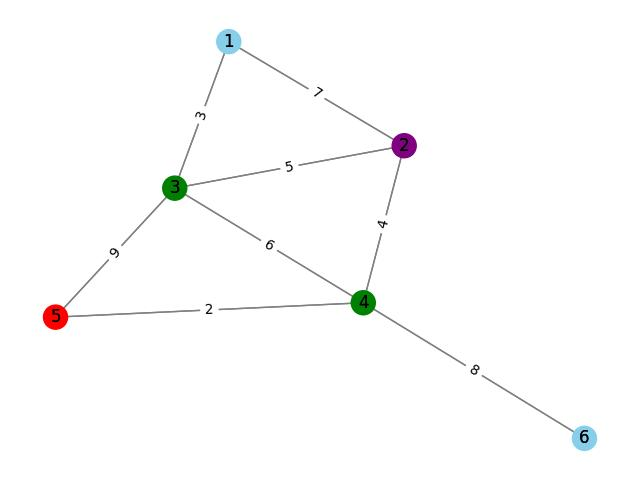
\includegraphics[width=0.75\textwidth]{7.jpg}
\caption{Park numer 7}
\end{figure}
\begin{figure}[h!]
\centering
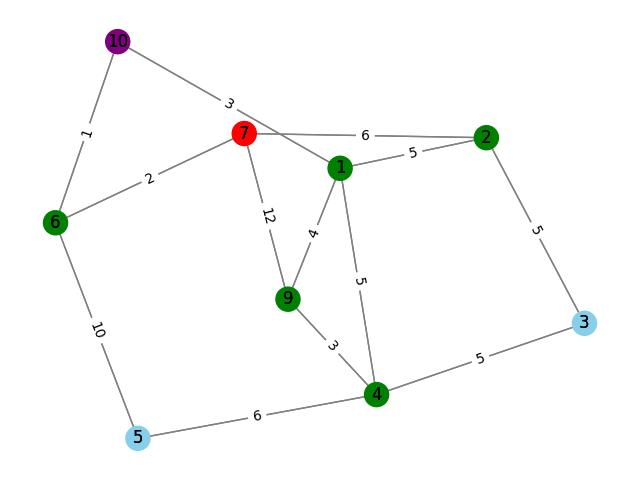
\includegraphics[width=0.75\textwidth]{8.jpg}
\caption{Park numer 8}
\end{figure}
\begin{figure}[h!]
\centering
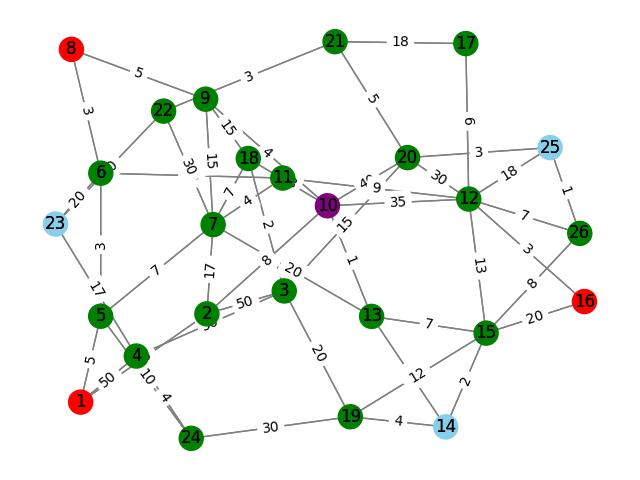
\includegraphics[width=0.75\textwidth]{9.jpg}
\caption{Park numer 9}
\end{figure}
Projekt zawiera rozszerzenia R0 i R1. Czyli moze sie znalezc pare wyjsc oraz pare osk. Pisany w javie, pythonie i bashu. Korzystamy ze struktury danych DS1. Wszystkie macierze sa zapamietywane jako mapa map i intow z wartosciami nierowynymi 0. 
\section{Hipoteza 1}
H1: Algorytm A2 zwykle daje dokladniejsze wyniki niz A1. Roznica dokladnosci rosnie wraz z rozmiarem macierzy i liczba niezerowych wspolczynnikow.
\begin{figure}[h!]
\centering
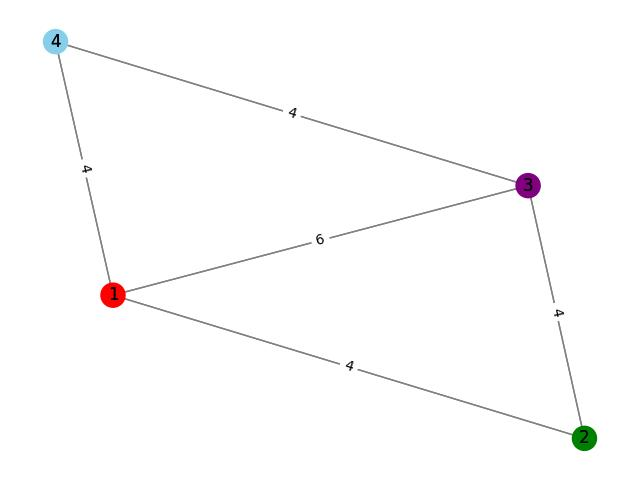
\includegraphics[width=0.75\textwidth]{1.jpg}
\caption{Park numer 1}
\end{figure}
\begin{figure}[h!]
\centering
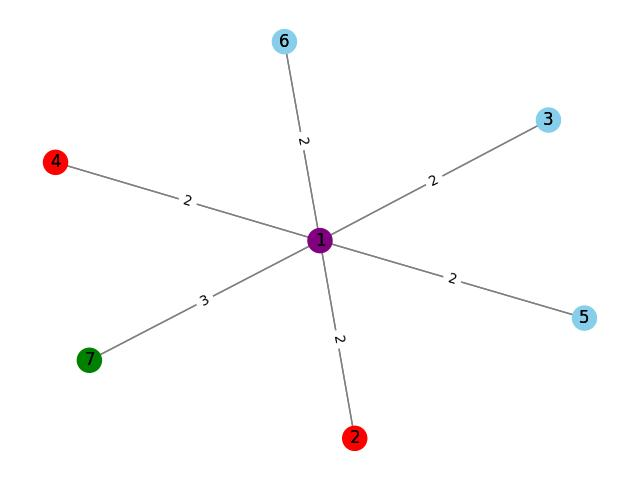
\includegraphics[width=0.75\textwidth]{2.jpg}
\caption{Park numer 2}
\end{figure}
\begin{figure}[h!]
\centering
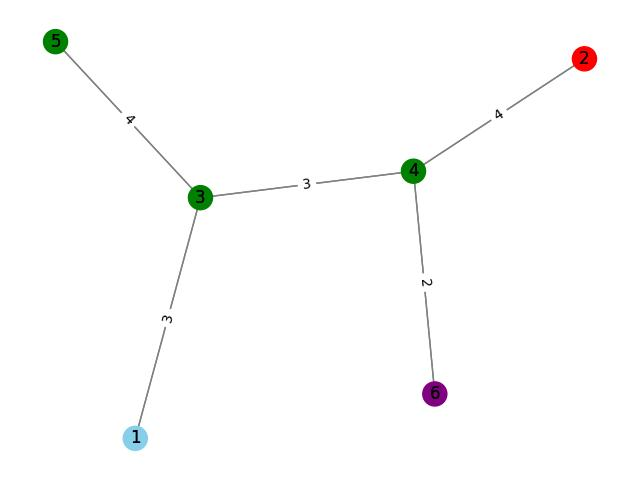
\includegraphics[width=0.75\textwidth]{3.jpg}
\caption{Park numer 3}
\end{figure}
\begin{figure}[h!]
\centering
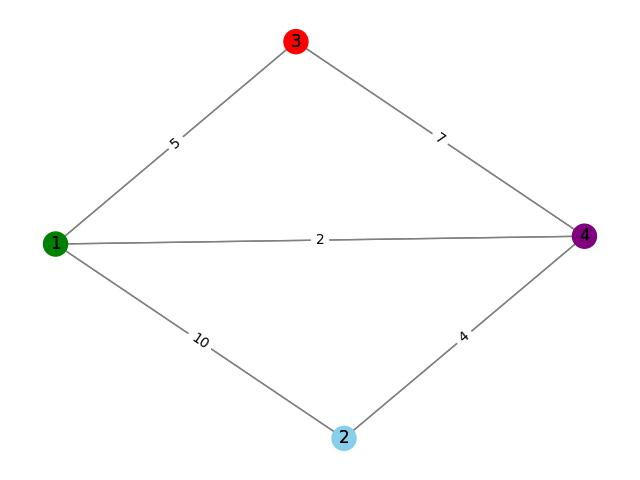
\includegraphics[width=0.75\textwidth]{4.jpg}
\caption{Park numer 4}
\end{figure}
\begin{figure}[h!]
\centering
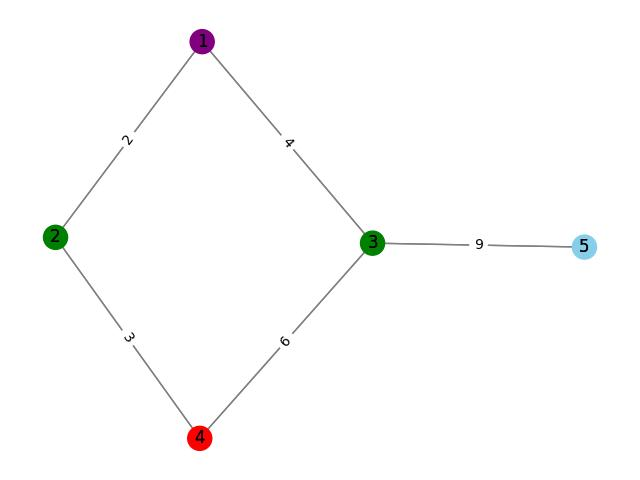
\includegraphics[width=0.75\textwidth]{5.jpg}
\caption{Park numer 5}
\end{figure}
\begin{figure}[h!]
\centering
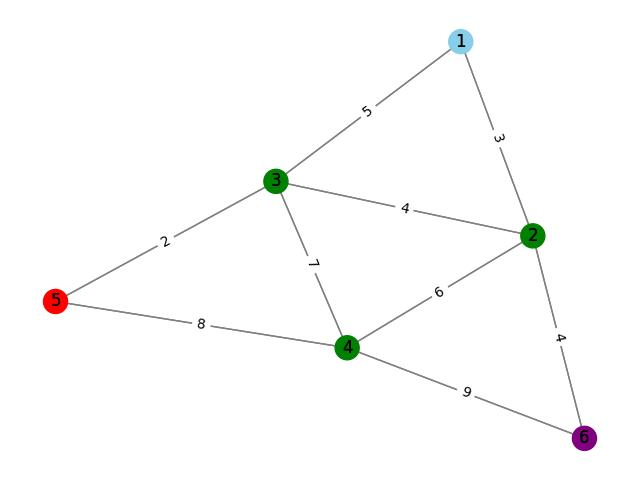
\includegraphics[width=0.75\textwidth]{6.jpg}
\caption{Park numer 6}
\end{figure}
\begin{figure}[h!]
\centering
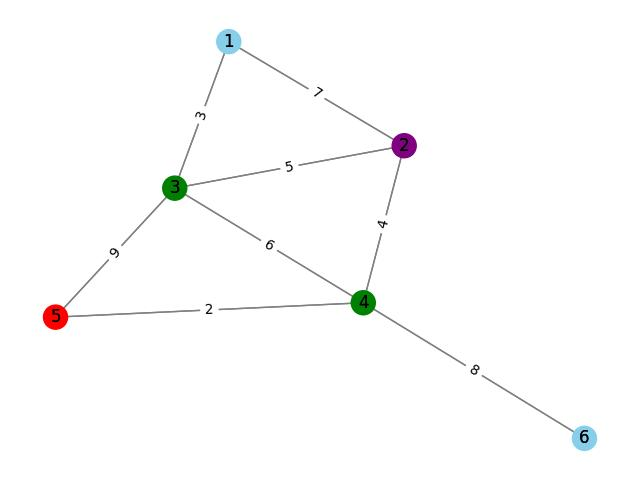
\includegraphics[width=0.75\textwidth]{7.jpg}
\caption{Park numer 7}
\end{figure}
\begin{figure}[h!]
\centering
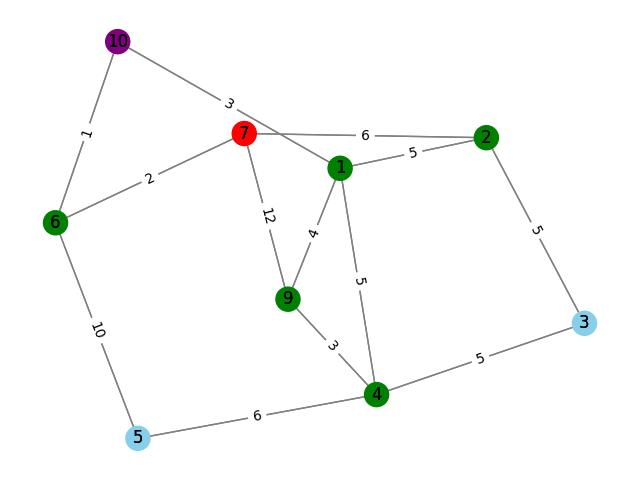
\includegraphics[width=0.75\textwidth]{8.jpg}
\caption{Park numer 8}
\end{figure}
\begin{figure}[h!]
\centering
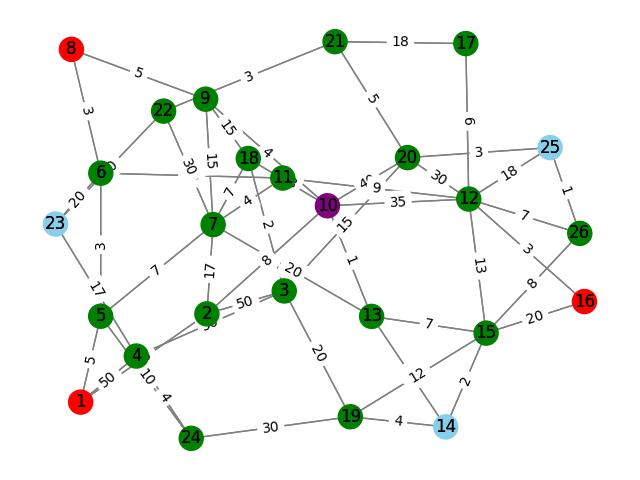
\includegraphics[width=0.75\textwidth]{9.jpg}
\caption{Park numer 9}
\end{figure}
Hipoteza nieprawdziwa. Dla kazdego przykladu wyniki otrzymywane byly takie same.
\section{Hipoteza 2}
H2: Algorytm A3 dziala dla postawionego zadania
???
\section{Hipoteza 3}
H3: Jesli algorytm A3 jest zbiezny do rozwiazania, to wyniki otrzymujemy istotnie szybciej niz dla A1 i A2
Hipoteza (nie)prawdziwa
\begin{figure}[h!]
\centering
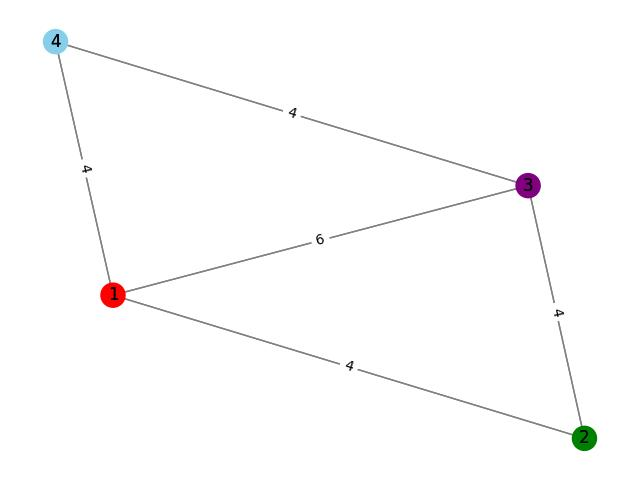
\includegraphics[width=0.75\textwidth]{1.jpg}
\caption{Park numer 1}
\end{figure}
\begin{figure}[h!]
\centering
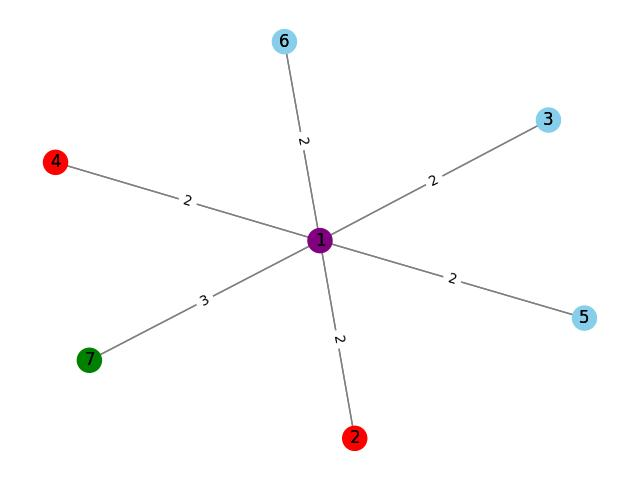
\includegraphics[width=0.75\textwidth]{2.jpg}
\caption{Park numer 2}
\end{figure}
\begin{figure}[h!]
\centering
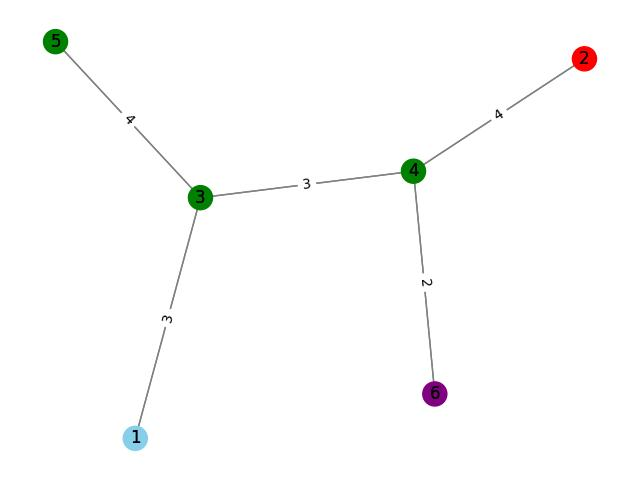
\includegraphics[width=0.75\textwidth]{3.jpg}
\caption{Park numer 3}
\end{figure}
\begin{figure}[h!]
\centering
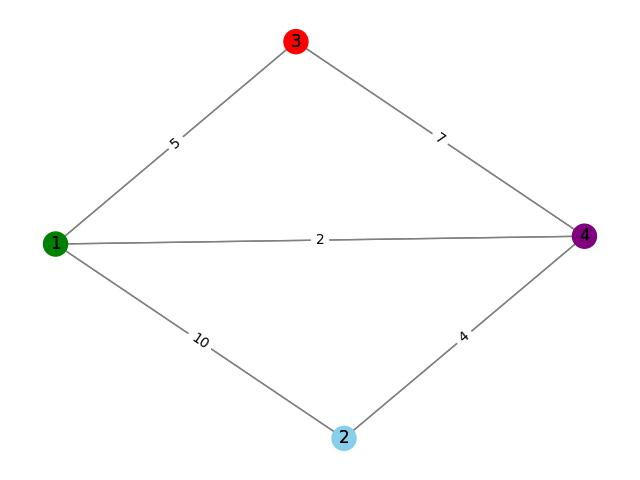
\includegraphics[width=0.75\textwidth]{4.jpg}
\caption{Park numer 4}
\end{figure}
\begin{figure}[h!]
\centering
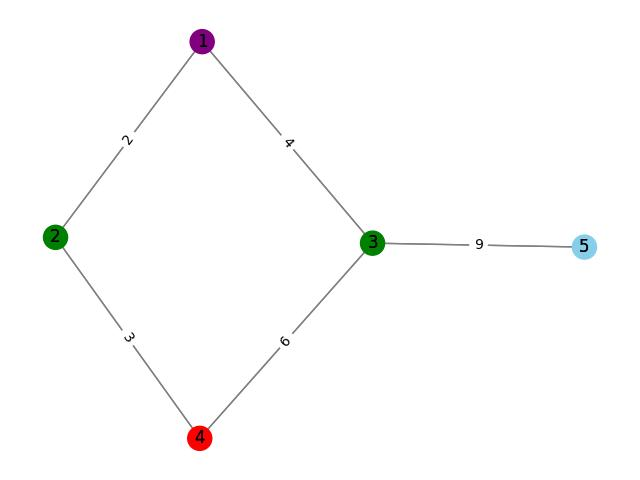
\includegraphics[width=0.75\textwidth]{5.jpg}
\caption{Park numer 5}
\end{figure}
\begin{figure}[h!]
\centering
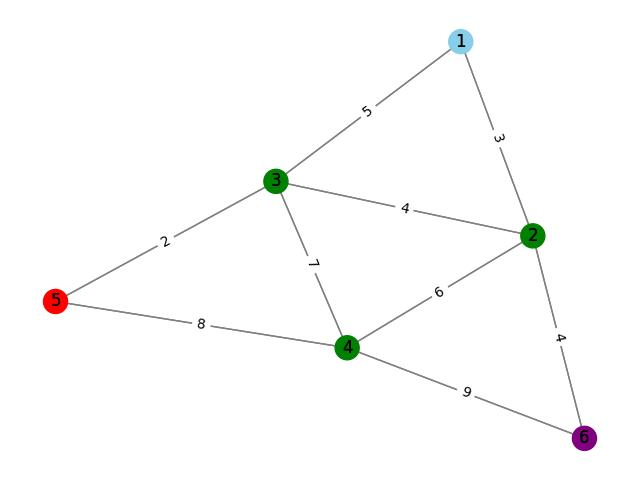
\includegraphics[width=0.75\textwidth]{6.jpg}
\caption{Park numer 6}
\end{figure}
\begin{figure}[h!]
\centering
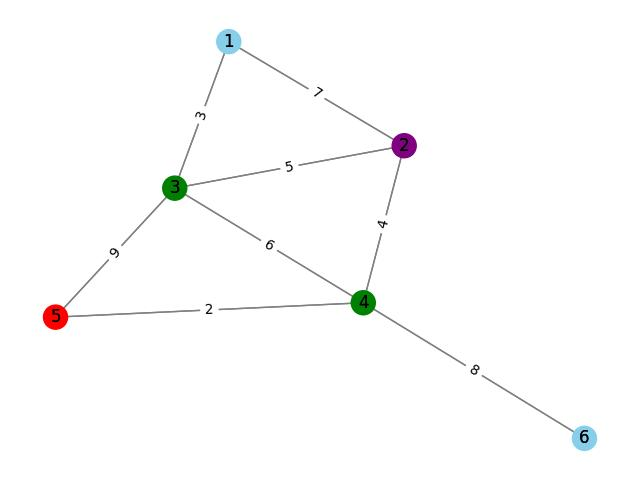
\includegraphics[width=0.75\textwidth]{7.jpg}
\caption{Park numer 7}
\end{figure}
\begin{figure}[h!]
\centering
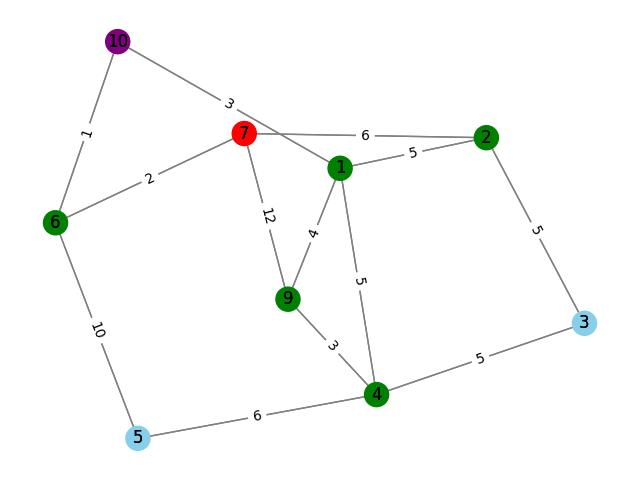
\includegraphics[width=0.75\textwidth]{8.jpg}
\caption{Park numer 8}
\end{figure}
\begin{figure}[h!]
\centering
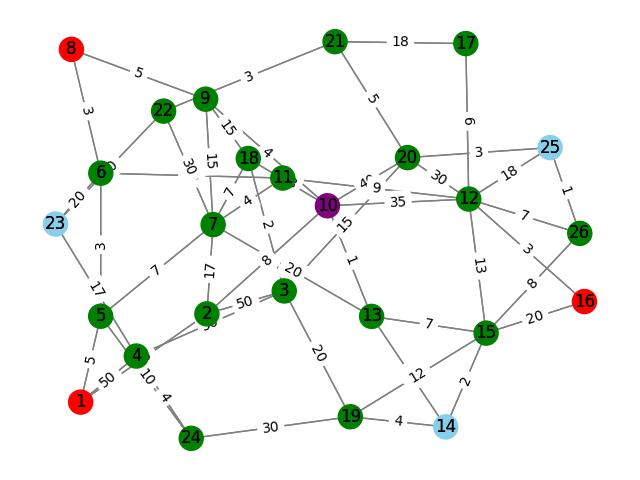
\includegraphics[width=0.75\textwidth]{9.jpg}
\caption{Park numer 9}
\end{figure}
\end{document}
